\documentclass{wyrmtongue-oct}
\usepackage[utf8]{inputenc}
\usepackage{xifthen}
\usepackage[super]{nth}
\usepackage{xcolor}
\usepackage{hyperref}
\usepackage{eso-pic}

\hypersetup{
    colorlinks=true,
    linkcolor=blue, 
    citecolor=black,
    urlcolor=blue,
    citecolor = blue,
    anchorcolor = blue
}

\begin{document}
% \thispagestyle{empty}
% \begin{center}
%     % 
\includegraphics[width=\textwidth]{img/profile/placeholder.png}
%     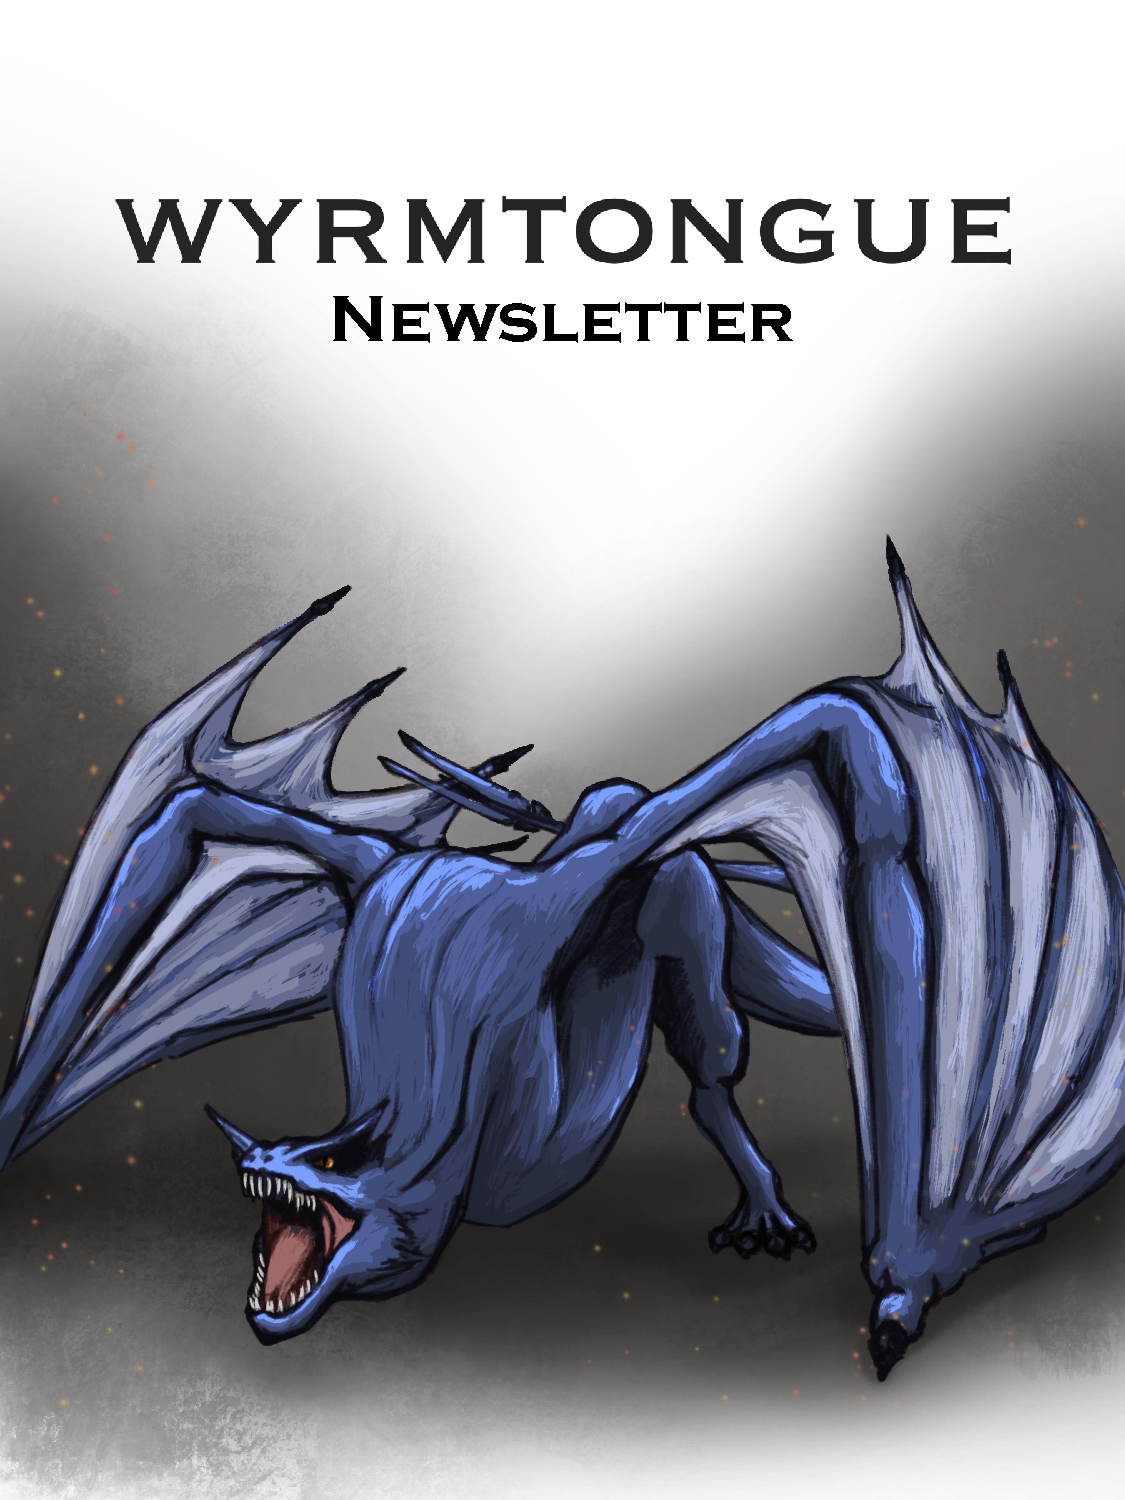
\includegraphics[width=\linewidth]{img/newsletter-cover-no-logo-2024.pdf}
% \end{center}
% \par\vspace{\fill}
% \begin{center}
%   
\includegraphics[width=0.4\textwidth]{img/logo/logo-alt.png}
% \end{center}

\begin{titlepage}
    \AddToShipoutPictureBG*{%
              \AtPageLowerLeft{%
                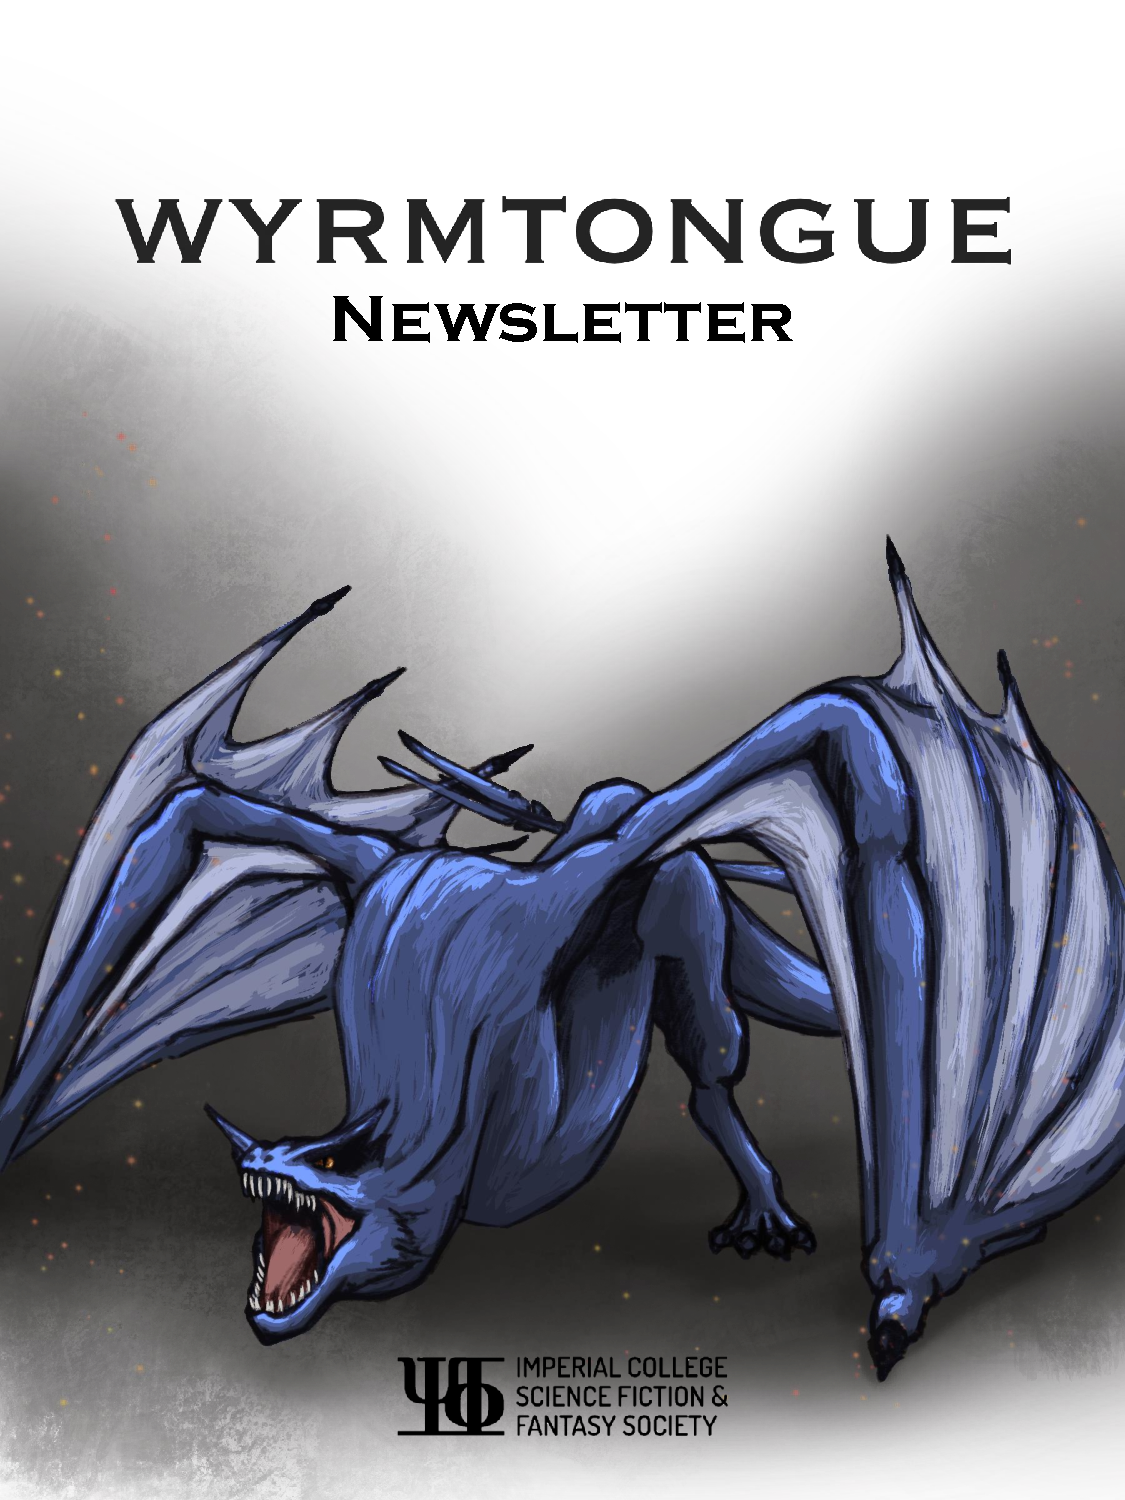
\includegraphics[width=\paperwidth,height=\paperheight]{img/newsletter-cover-2024.pdf}%
              }%
            }
\end{titlepage}

\textbf{      } % this is so hacky

\clearpage
\setcounter{page}{1}

\tableofcontents
\clearpage

% \pagehead{README}
To the unfortunate souls who chose to work on this mess of a template, here's what you need to do:

\begin{enumerate}
    \item Navigate to the \verb|txt| folder. You should find a .tex file named after your role. Type your stuff on there.
    \item Once that's done, pick an appropriate profile picture and head to the \verb|profile| folder under \verb|img|. Rename your picture with one of the png file names and replace it.
    \item Go to \verb|main.tex| and replace ``placeholder" with the appropriate tag in your section ie ``chair" or ``librarian"
\end{enumerate}

Note: If you face any issues, please harass the dumbass who got elected to be editor this year. Happy \LaTeX ing :)\
\clearpage

\article{editor}{From the Editor}
{Clifford Chan}{Editor}
\footnotetext[2]{Check out the Picocon section to find out more :)}
\clearpage

\article{chair}{Captain's Log}
{Hazel Wright}{Chair Entity}
% \footnotetext[2]{The Chair Entity is watching you.}
\clearpage

\article{librarian}{Welcome to the Library!}
{Kai Lam}{Head Librarian}
% \clearpage
\vspace{3em}

\pagehead{Book Recommendations}

If you're looking to dive into the library's collection but are having
trouble deciding where to start, here are some recommendations from
the committee:

\bookrec{Ash Robson}{The Expanse Series}{James S A Corey}{Hard Sci-Fi with brilliant action, tense interplanetary politics, a hard-boiled detective, and of course a spooky alien virus. Couple that with some great writing and you can understand why I read the first book in a day and a night (sleep is for the weak!)}

\bookrec{Clifford Chan}{The Three Body Problem}{Liu Cixin}{The first of a mind bending hard sci-fi trilogy that won the Hugo Award in 2015. Also has a decent Netflix adaptation!}

\bookrec{Clifford Chan}{The Way of Kings}{Brandon Sanderson}{Beginning with the assassination of a king, this is a tale of a slave breaking free of his chains. One of Sanderson's greatest works to date, and the beginning of the Stormlight Archives. You're in for a storming treat.}

\bookrec{Clifford Chan}{The Grace of Kings}{Ken Liu}{Described as silkpunk fantasy, two brothers lead their seperate rebellions against the emperor of Dara. Inspired by real historical events, namely the Chu-Han Contention, this is a must-read for fans of epic fantasy.}

\bookrec{Clifford Chan}{The Wheel of Time series}{Robert Jordan}{At times tedious, this 14-book spanning story is one of gargantuan proportions. While rather trope-y, the series boasts great characters and a plot that, despite its meandering nature, reaches heights of awesome I didn't know was possible.}

\bookrec{Kai Lam}{The Fifth Science}{Exurb1a}{A whimsical look at the effects "the fifth science" has on the future of humankind. So good I'm giving my copy to the library so more people read it.}

\bookrec{Kai Lam}{His Dark Materials}{Philip Pullman}{Not a high-concept fantasy but with interesting philosophy and a great adventure.}

\bookrec{Kai Lam}{The Long Earth series}{Terry Pratchett and Stephen Baxter}{Great concept and execution, where it's possible to step into parallel worlds.}

\bookrec{Kai Lam}{Keys to the Kingdom Series}{Garth Nix}{A boy saves the universe story that I found a fun read.}
\clearpage

\article{events}{Events}
{Juairiyah Raqib}{Chair of Vice\\(Events Officer)}
\clearpage

% Would the publicity officer(Michelle) need a page?

% % wanted to do some fancy macro things to make this not tedious, but it's
% Tuesday on the week of Picocon and I am panicking.
\newcommand{\mtr}[2]{ \multirow{#1}{*}{\parbox{0.6\textwidth}{#2}} }
\newcommand{\tevent}[3]{
  {#1} \textbf{#2} \par \vspace{0.1\baselineskip}{\footnotesize #3} \par
}

\begin{center}
  \begingroup
  \renewcommand*{\arraystretch}{2.3}
  \begin{tabular}[t]{p{0.1\textwidth} l}
    \hline
    \texttt{09:00} &
    \tevent{Front Desk / registration opens}{}{} \\ \cline{2-2}

    \texttt{10:00} &
    \mtr{2}{
      \tevent{Guest Talk:}{James Flanagan}{Blackett Bulding LT2}
    } \\
    \texttt{10:55} & \\ \cline{2-2}

    \texttt{11:00} &
    \mtr{2}{
      \tevent{Guest Talk:}{qntm}{Blackett Building LT2}
    } \\
    \texttt{11:55} & \\ \cline{2-2}

    \texttt{12:00} &
    \mtr{2}{
      \tevent{Guest Talk:}{Kevin Jon Davies}{Blackett Building LT2}
    } \\
    \texttt{12:55} & \\ \cline{2-2}

    \texttt{13:00} &
    \mtr{2}{
      \tevent{}{LUNCH}{Nourish thy mind and body...}
    } \\
    \texttt{13:55} & \\ \cline{2-2}

    \texttt{14:00} & 
    \mtr{3}{
      \tevent{}{Destruction of dodgy merchandise}{Queen's Lawn}
      \tevent{}{Baguette Bash}{Queen's Lawn}
    } \\ \\
    \texttt{14:55} & \\ \cline{2-2}

    \texttt{15:00} &
        \mtr{2}{
          \tevent{}{Guest of Honour Q\&A Panel}{Blackett Building LT2}
        } \\
        \texttt{15:55} & \\ \cline{2-2}

    \texttt{16:00} &
    \mtr{2}{
      \tevent{}{Turkey Talks}{Blackett Building LT2}
    } \\
    \texttt{17:55} & \\ \cline{2-2}
    
    \texttt{18:00} &
    \mtr{2}{
      \tevent{}{The Picocon Quiz}{Blackett Building LT2}
    } \\
    \texttt{19:00} & \\ \hline
  \end{tabular}
  \endgroup
\end{center}

% \footnotetext[2]{Continues into the week --- drop by the library whenever
%   and pick up a mystery book.}
% \footnotetext[3]{Themed Fridays usually start at 18:00 in the Library.}
% \footnotetext[4]{Extraordinary General Meeting. Run for a committee position!}
\clearpage

\article{picocon}{Picocon}
{Ash Robson}{Picocon Sofa}
% \footnotetext[2]{source: me, I thought about it}
\footnotetext[3]{Guests of Honour to be announced in the coming months, stay tuned}
\footnotetext[4]{no guarantee your psyche will leave unharmed}
\clearpage

% \pagehead{Picocon Sneak Peek!!}

\begin{center}
    
\includegraphics[height=\textwidth]{img/profile/placeholder.png}
\end{center}

We also publish a collection of short stories, artwork and poetry in conjunction with Picocon! This year's theme is \textit{???}. If you wish to contribute to the fanzine, submit your work to \texttt{icsfwyrmtongue@gmail.com}\footnotemark[2]. 

% \footnotetext[2]{Submissions will be open from start of Spring term until ???.}
% \clearpage

% \pagehead{Whispers from the Basement}

Imperial College Science Fiction and Fantasy Society brings their
weird and wonderful conversations directly to your auditory organs!
Tune in for an hour of terrible banter, mysterious music, and
life-changing revelations in dialogue.

\textit{Whispers from the Basement} airs every Wednesday afternoon
14:00--15:00 on IC Radio. Find updates about the show and listen to
previous broadcasts on the IC Radio website
at \texttt{icradio.com/shows/1016/}.

% \par\vspace{\fill}
\pagehead{Getting Involved}

\subhead{Mailing Lists}

ICSF maintains the following mailing lists, to which all members are welcome to
subscribe:

\begin{itemize}
\item \texttt{icsf-list}
is the society’s core mailing list, which communicates announcements
of ICSF events and important news about the society. This list does
not generate an overwhelming amount of traffic, and subscription is a
must if you would like to hear about film trips and other activities.

% \item \texttt{icsf-committee}
% is our ‘management’ list --- but it gets used a lot more
% widely than that. Here you’ll be able to contribute your opinion to
% the running of the society.
\end{itemize}

% QR code for mailing list
\begin{minipage}[h]{7.8em}

\includegraphics[height=\textwidth]{img/info/qr-mailing-list.png}
\end{minipage}
\begin{minipage}[h]{0.82\linewidth}
\raggedright
Join our mailing list by scanning the QR code. Alternatively, subscribe automatically by signing up for membership at: 
\href{https://www.imperialcollegeunion.org/activities/a-to-z/science-fiction-and-fantasy}{www.imperialcollegeunion.org/activities/a-to-z/science-fiction-and-fantasy}.
\end{minipage}

\subhead{Social Media}
For those who welcome our social network overlords, behold
continuations of the Library into the realms of cyberspace:

\socialmedia{facebook}{\href{https://www.facebook.com/groups/ICSF.imperial}{facebook.com/groups/ICSF.imperial}}{
Sci-fi talk, news and events, amusing links.
}

% \socialmedia{twitter}{@Picocon}{
% Announcements and excitement for our annual convention.
% }

\socialmedia{twitter}{\href{https://twitter.com/Imperial_SciFi}{@Imperial\_SciFi}}{
Sci-fi and fantasy, 280 characters at a time.
}

\socialmedia{instagram}{\href{https://www.instagram.com/imperial_scifi/?hl=en}{@imperial\_scifi}}{
Visions from the library, visions from the future (event announcements).
}

\par\vspace{\fill}
\clearpage

% \pagehead{\LARGE Book review -- Neuromancer by William Gibson}
Things to write here...
% \tombstone
% \clearpage

% %\begin{Puzzle}{22}{22}
%|{} |{} |{} |{} |{} |{} |{} |{} |{} |[1]B |U |B |[2]B |L |[3]E |G |U |[3]M|.
%|{} |{} |{} |{} |{} |{} |{} |{} |{} |{} |{} |{} |A|{} |{} |{} |{} |I |.
%|{} |{} |{} |{} |[4]N |{} |[5]S |{} |{} |[6]A |N |A |R |C |H |Y |{} |R |.
%|{} |{} |{} |{} |O |{} |E |{} |{} |{} |{} |{} |A |{} |{} |{} |{} |A |{} |[7]M |.
%|[8]C |A |D |I |A |{} |L |{} |{} |{} |{} |{} |D |{} |{} |{} |{} |N |{} |A |.
%|R |{} |{} |{} |H |{} |[9]D |E |A |T |H |{} |[10]D |O |M |E |S |D |A |Y |.
%|E |{} |{} |{} |{} |{} |O |{} |{} |{} |{} |{} |U |{} |{} |{} |{} |A |* |A|.
%|[11]T |H |E |R |M |O |N |[12]U |C |L |E |[13]A |R |{} |{} |{} |{} |{} |[14]T |.
%|A |{} |{} |{} |{} |{} |{} |F |{} |{} |{} |L |{} |{} |{} |{} |{} |{} |H |.
%|C |{} |{} |{} |{} |{} |[15]B |O |[16]R |G |{} |[17]D |E |A |T |H |S |T |A |R |.
%|[18]E |L |D |A |[19]R |{} |{} |{} |E |{} |{} |E |{} |{} |{} |{} |{} |{} |N |.
%|O |{} |{} |{} |E |{} |[20]B |{} |M |{} |{} |R |{} |[21]W |{} |{} |{} |{} |O |.
%|U |{} |{} |{} |A |{} |O |{} |{} |{} |[22]F |A |M |I |N |E |{} |{} |S |.
%|S |{} |{} |{} |P |{} |T |{} |{} |{} |{} |A |* |N |. 
%|{} |{} |{} |{} |[23]E |X |T |E |[24]R |M |I |N |A |T |E |{} |{} |[25]Z |.
%|{} |{} |[26]W |A |R |* |L |* |A |{} |{} |{} |{} |E |{} |{} |{} |O |{} |{} |{} |[27]E |.
%|{} |{} |{} |{} |{} |[28]B |E |R |G |{} |[29]N |E |C |R |O |N |O |M |I |C |O |N |.
%|{} |{} |{} |{} |{} |{} |C |{} |N |{} |{} |{} |{} |{} |{} |{} |{} |B |{} |{} |{} |T |.
%|{} |{} |{} |{} |{} |{} |A |{} |A |{} |{} |{} |{} |{} |{} |{} |[30]S |I |G |M |A |R |.
%|{} |{} |{} |{} |{} |{} |P |{} |R |{} |{} |{} |{} |{} |{} |{} |{} |E |{} |{} |{} |O |.
%|{} |{} |{} |{} |{} |{} |{} |[31]C |O |N |Q |U |E |S |T |{} |{} |S |{} |{} |{} |P |.
%|{} |{} |{} |{} |{} |{} |{} |{} |K |{} |{} |{} |{} |{} |{} |{} |{} |{} |{} |{} |{} |Y |.
%\end{Puzzle}

\begin{Puzzle}{12}{13}
|[1]H   |O      |B      |[2]B   |*      |[3]J   |A      |[4]R   |*      |[5]O   |R      |[6]C   |.
|O      |*      |*      |[7]O   |R      |A      |*      |[8]I   |O      |N      |*      |U      |.
|[9]G   |R      |O      |T      |*      |N      |*      |F      |*      |[10]I  |N      |T      |.
|S      |*      |*      |*      |[11]M  |E      |N      |T      |[12]A  |T      |*      |*      |.
|W      |*      |*      |[13]M  |I      |T      |*      |*      |V      |*      |*      |[14]C  |.
|[15]A  |T      |U      |I      |N      |*      |[16]H  |O      |A      |R      |A      |H      |.
|T      |*      |*      |D      |*      |[17]M  |E      |*      |L      |*      |*      |A      |.
|[18]C  |A      |N      |A      |L      |S      |*      |[19]D  |O      |W      |E      |L      |.
|H      |*      |*      |I      |*      |*      |[20]E  |O      |N      |*      |*      |C      |.
|*      |*      |[21]V  |R      |[22]I  |S      |K      |A      |*      |*      |*      |E      |.
|[23]E  |L      |L      |*      |A      |*      |A      |*      |[24]S  |A      |N      |D      |.
|G      |*      |[25]A  |R      |G      |*      |[26]N  |E      |O      |*      |*      |S      |.
|[27]O  |O      |D      |*      |[28]O  |K      |S      |*      |[29]L  |O      |S      |T      |.
\end{Puzzle}

\newcommand{\blnk}{\underline{\hspace{2em}}}

\newcommand{\cwclue}[4]{
% #1 - number
% #2 - answer
% #3 - question
% #4 - length
\item[\texttt{#1}] {{#3} ({#4})}
}
\hfill
\begin{minipage}[t]{0.45\textwidth}
\begin{center}{\large \altfont{Across}}\end{center}
\begin{small}
\begin{itemize}[leftmargin=*,topsep=0pt,itemsep=0pt]
\cwclue{1}{HOBB}{Following Robin, writer of 15 fantasy books set in and aorund the six Duchies.}{4}
\cwclue{3}{JAR}{Times two plus Binks.}{3}
\cwclue{5}{ORC}{In the Lord of the Rings, a grown up 9 Across.}{3}
\cwclue{7}{ORA}{Japanese for 'come on' oft shouted by muscular men beating eachother up.}{3}
\cwclue{8}{ION}{Common Sci-Fi cannon ammo.}{3}
\cwclue{9}{GROT}{In Warhammer, a younger 5 Across.}{4}
\cwclue{10}{INT}{Abbr. for a wizard's key trait.}{3}
\cwclue{11}{MENTAT}{Thufir Hawat is one example.}{6}
\cwclue{13}{MIT}{Where the newest Spiderman was rejected from.}{3}
\cwclue{15}{ATUIN}{A turtle upon whose sex lies the fate of millions}{5}
\cwclue{16}{HOARAH}{Godfrey, the First Elden Lord's other name.}{6}
\cwclue{17}{ME}{An immortal Viking met by the Doctor.}{2}
\cwclue{18}{CANALS}{What early Sci-Fi authors thought were on Mars.}{6}
\cwclue{19}{DOWEL}{Wooden furniture fasteners, the Sci-Fi Library may have a few.}{5}
\cwclue{20}{EON}{The world was young and magical a few of these ago.}{3}
\cwclue{21}{VRISKA}{The ever controversial arachnid from Homestuck}{6}
\cwclue{23}{ELL}{Mario's brother's letter.}{3}
\cwclue{24}{SAND}{Arrakis' truly most abundant resource.}{4}
\cwclue{25}{ARG}{(Acronym) Form of Youtube horror closely associated with conspiracy}{3}
\cwclue{26}{NEO}{Mr. Anderson's other, true name.}{3}
\cwclue{27}{OOD}{Tentacled enemy of the Doctor.}{3}
\cwclue{28}{OKS}{Vader does this to the destruction of Alderaan.}{3}
\cwclue{29}{LOST}{A 2004 American TV show inspired by Cast Away}{4}
\end{itemize}
\end{small}
\end{minipage}
\hfill
\begin{minipage}[t]{0.45\textwidth}
\begin{center}{\large \altfont{Down}}\end{center}
\begin{small}
\begin{itemize}[leftmargin=*,topsep=0pt,itemsep=0pt]
\cwclue{1}{HOGSWATCH}{Discworld's most popular Holiday}{9}
\cwclue{2}{BOT}{Asimov's specialty}{3}
\cwclue{3}{JANET}{A soon to be Mrs. Majors from the Rocky Horror Picture Show.}{5}
\cwclue{4}{RIFT}{Setting in which League of Legends' battles occur.}{4}
\cwclue{5}{ONIT}{Where a Sci-Fi book is kept in relation to its bookshelf.}{4}
\cwclue{6}{CUT}{What many fans wish to do to George Lucas' various changes to Star-Wars.}{3}
\cwclue{11}{MIN}{An abbreviation for least (I tried but I couldn't think of a sci-fi related clue)}{3}
\cwclue{12}{AVALON}{Island of magic, where Caledfwlch was forged.}{6}
\cwclue{13}{MIDAIR}{The setting for the movie Airplane}{6}
\cwclue{14}{CHALCEDST}{The slaver kingdom in 1 Across' series.}{9}
\cwclue{16}{HE}{Followed by Man, fights the evil forces of Skeletor.}{2}
\cwclue{17}{MS}{Followed by paint, a webcomic artist's easel.}{2}
\cwclue{19}{DOA}{Acronym for the 3D fighting game of '96.}{3}
\cwclue{20}{EKANS}{Creatively named slithery Pokemon}{5}
\cwclue{21}{VLAD}{Romania's famed impaler, Whitby's famed blood-sucker.}{4}
\cwclue{22}{IAGO}{Agrabah's famous Parrot, owned by Jafar.}{4}
\cwclue{23}{EGO}{The Lord of the stars' Father.}{3}
\cwclue{24}{SOL}{Our Sun's name}{3}
\end{itemize}
\end{small}
\end{minipage}
\hfill

% Wukong   A monkey born out of a magic stone
% Minotaur Guardian of the labyrinth
% Banshee  An Irish fairy whose screams are regarded as a portent of death
% Dullahan A headless horseman from Irish folklore
% Phoenix  Dumbledore's pet
% Selkie   Celtic seal people
% Naga     Half-human, half-serpent creatures of the netherworld
% Wyvern   A dragon with two legs
% Cthulu   A high priest of the Great Old Ones
% Kitsune  A fox spirit of Japanese origin
% Hydra    A many-headed snake
% Goblin   Every D&D party's first enemy (they're green)
% Kraken   A gigantic cephalopod
% Cyclops  One-eyed giants
% Sphinx   Answer me riddle...


% \clearpage

\vspace*{\fill}
\begin{center}
  
\includegraphics[width=0.3\textwidth]{img/qr-small.png} \par
  February 2019 \textemdash{} \texttt{icsf.org.uk}
\end{center}
\vspace*{4\baselineskip}

\clearpage

\end{document}
